% !TEX root = ../thesis.tex
\section{Získání sekvence pozorování}
\label{chap:asr:parametrization}

Jako v mnoha jiných odvětvích, tak i při rozpoznávání řeči je v mnoha případech inspirací člověk. Pro získání sekvence pozorování (příznaků) vycházíme z \textbf{modelování produkce řeči} a \textbf{modelování procesu slyšení}, které se inspirují právě člověkem.

\subsection{Modelování produkce řeči}
\label{chap:asr:parametrization:production}

Cílem modelování produkce řeči je nalezení matematických vztahů, které poslouží k reprezentaci fyzikálních dějů spojených s produkcí řeči. Základem je parametrizační technika \textbf{lineárního prediktivního kódování}, známá pod anglickou zkratkou LPC\footnote{Linear Predictive Coding} \cite{Benesty2007}. Vychází z představy, že hlasové ústrojí člověka je schopno vytvářet tři různé typy řečových zvuků:

\begin{itemize}
  \item \textit{samohlásky} - ty se řadí mezi znělé typy zvuků produkované periodickým buzením vznikajícím pulsy vzduchu, které jsou produkovány hlasivkami;
  \item \textit{frikativy} (např. $/f/$\footnote{Zápis $/f/$ symbolizuje foném, což je akustická reprezentace písmene, \textit{f}. Konkrétní zápisy se mohou lišit podle použité fonetické abecedy. V Čechách se nejčastěji používá abeceda $SAMPA$ či $Z\check{C}FA$.}) - někdy nazývané jako třené souhlásky, protože vznikají třením výdechovaného proudu vzduchu o překážku v některém místě hlasového ústrojí. Těmito překážkami může být jazyk, zuby ap.;
  \item \textit{explozivy} (např. $/b/$, $/p/$ ap.) - také nazývané jako souhlásky výbuchové, se tvoří úplnýn uzavřením vydechovaného proudu vzduchu pomocí artikulačních orgánů. To se následně projeví jako krázká pauza (tzv. okluze), po které následuje náhlé jednorázové uvolnění a únik nahromaděného vzduchu, tzv. exploze \cite{Psutka2006};
\end{itemize}

Snahou modelování je navržení modelu hlasového traktu, který bude dobře popisovat výše popsané zvuky. Nesmí se všask zapomenout na možnou složitost a přesnost modelu, jako ideální by byl linéárně časově invariantní model. Bohužel lidská řeč představuje kontinuální časově variantní a v některých situacích dokonce nelineární proces, takže je téměř nemožné jej přesně namodelovat. Pokud se včask udělají určité rozumné předpoklady, tak možné navrhnout lineární časově invariantní model řeči platný pro krátké časové úseky. Jinými slovy, předpokladem je, že v tomto krátkém časovém zůstává buzení a parametry hlasivkového traktu přibližně konstantní. Tento předpoklad přibližně platí pro intervaly $10$ až $30\ ms$. Odtud také vychází uvažovaná perioda segmntů řeči, viz úvod této kapitoly. Za těchto okolností je možné proces vytváření řeči modelovat pomocí tzv. \textbf{krátkodobého modelu}, který má v krátkých časových intervalech pevné parametry \cite{Holmes2001}.

\begin{figure}[hbpt]
  \centering
  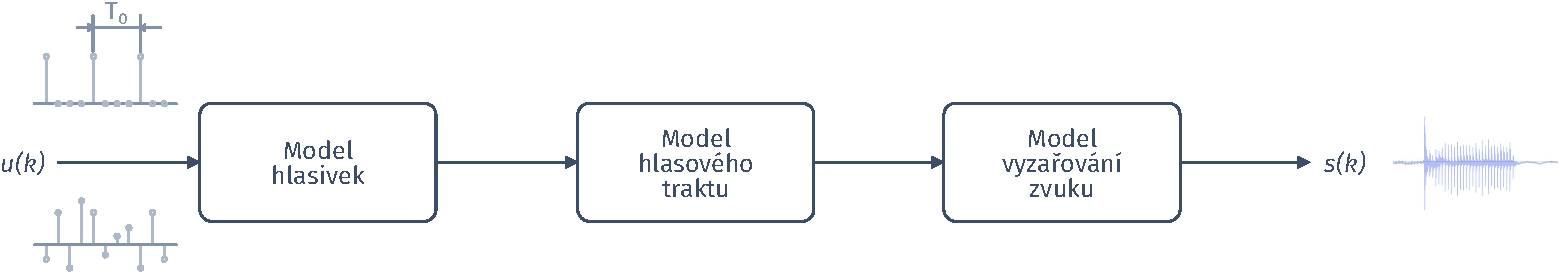
\includegraphics[width=0.9\textwidth]{./ch4-asr/img/speech_model.pdf}
  \caption{Blokové schéma modelu produkce řeči}
  \label{fig:asr:model:speech}
\end{figure}

Pro odvození obecného diskrétního modelu hlasovkového traktu se vychází ze zjednodušeného modelu produkce řeči (obr. \ref{fig:asr:model:speech}). Ten je tvořen modelem hlasivek, modelem hlasivkového traktu a modelem vyzařovaného zvuku, které jsou seriově řazeny. K odvození a popisu vlastností modelu se využívá výhod z-transformace \cite{Psutka2006}. Po zjednodušení je krátkodobý model produkce řeči aproximovat celopólovým modelem (filtrem) $H(z)$ ve tvaru

\begin{equation}
  H(z) = \frac{G}{1 + \sum_{i = 1}^{Q} a_{i} z^{-i}} = \frac{S(z)}{U(z)},
  \label{eq:asr:lpc:generic}
\end{equation}

\noindent kde $G$ představuje celkové zesílení, $Q$ je řád modelu odpovídající $2K + 1$ počtu formantů, které má model postihovat, $a_i$ jsou parametry modelu. Vstupem modelu je buzení $u(k)$ (viz obr. \ref{fig:asr:model:speech}), tedy pro znělé zvuky sled pulsů s periodou $T_0$\footnote{Prioda základního hlasivkového tónu.} a pro neznělé zvuky náhodný šum s plochým spektrem. V časové oblasti je pak diskrétní výstupní odezva při fixovaných parametrech hlasového traktu ($10 - 30\ ms$) dána konvolucí a buzení a impulzní odezvy krátkodobého modelu. Na základě toho je možné model upravit na tvar podle obr. \ref{fig:asr:model:speech:excitation}, kde je $u(k)$ buzení a $s(k)$ je výstupní signál s parametry hlasového ústrojí odpovídající $a_i$ celopólového modelu.

\begin{figure}[hbpt]
  \centering
  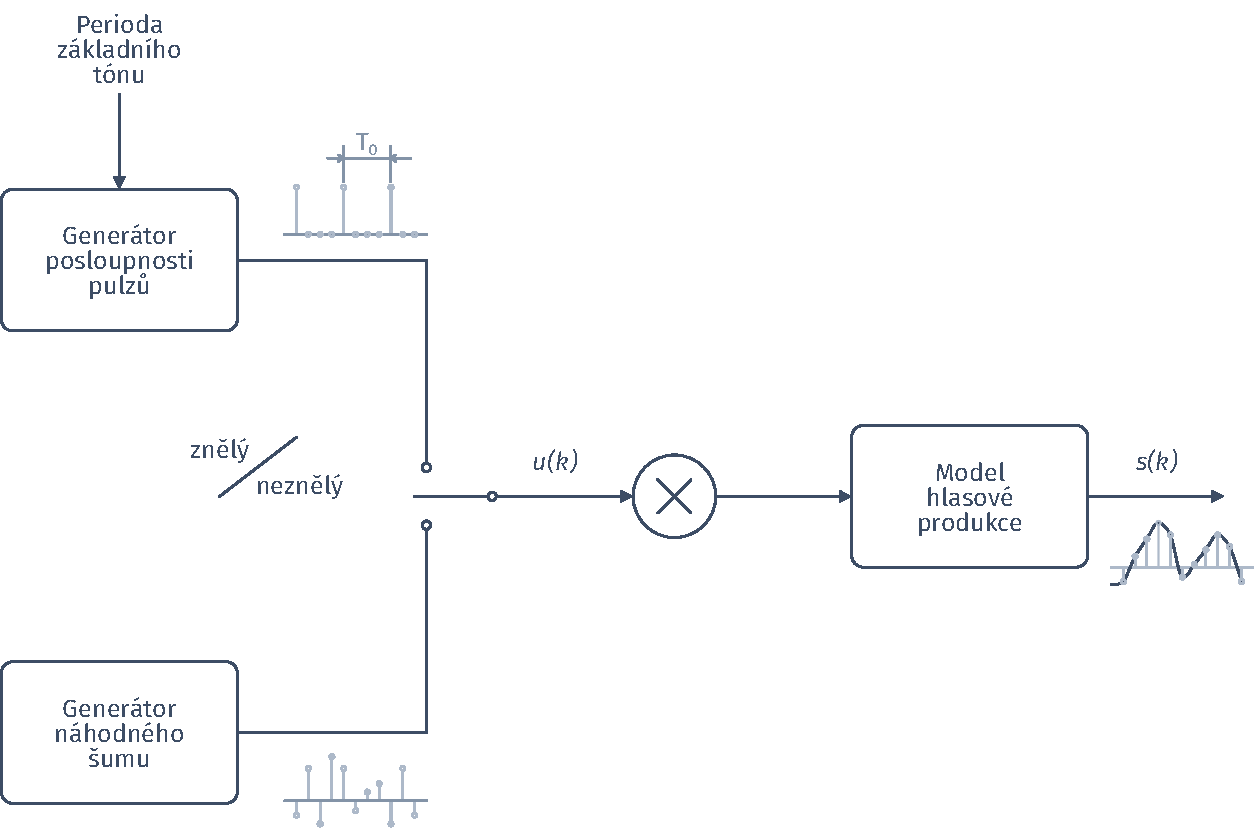
\includegraphics[width=0.9\textwidth]{./ch4-asr/img/speech_process.pdf}
  \caption{Blokové schéma upraveného modelu produkce řeči}
  \label{fig:asr:model:speech:excitation}
\end{figure}

K odhadu parametrů $a_i$ slouží \textbf{lineární prediktivní analýza}. Odhad probíhá přímo z krátkodobého řečového signálu. Přenosové vlastnosti krátkodobého modelu je možné popsat rovnicí (\ref{eq:asr:lpc:generic}). Myšlenka metody LPC staví na předpokladu, že vzorek $k$ řečového signálu je možné popsat lineární kombinací $Q$ předchozích vzorků a buzení $u(k)$, což lze zapsat úpravou vztahu (\ref{eq:asr:lpc:generic}) do tvaru

\begin{equation}
  s(k) = - \sum_{i = 1}^{Q} a_i s(k-1) + Gu(k).
\end{equation}

\noindent Z něj je atrné, že se LPC snaží parametry modelu $a_i$ a zesílení $G$ odhadnout pomocí známe reálně naměřené posloupnosti $s(k)$. K vyřešení se používá principu minimalizace kvadratické chyby krátkodobé energie signálu. Ta je v časové oblasti popsána vztahem

\begin{equation}
  E = \sum_{k} e^2(k) = \sum_{k} \left[ s(k) - s'(k)\right]^2 = \sum_{k} \left( s(k) + \sum_{i = 1}^{Q} a_i s(k-1) + Gu(k) \right),
\end{equation}

\noindent kde $s(k)$ jsou vzorky reálného řečového signálu a $s'(k)$ jsou ty predikováné LPC filtrem. K získání řešení krátkodobé chyby predikce $E$, pro konkrétní analyzovaný segment, je použita metoda nejmenších čtverců. K výpočtu konkrétních koeficientů modelu $a_i$ je možné použít rekurzivního Durbinova algoritmu \cite{Holmes2001}.

Další možností jak popsat hlasový trakt je pomocí \textbf{kepstrálních koeficientů lineární predikce}. Kepstrum je definováno jako inverzní diskrétní Fourierova transformace (IDFT) logaritmu velikosti transformovaného vstupního signálu pomocí diskretní Fourierovy transformace (DFT), matematicky popsáno vzhaem

\begin{equation}
  c(k) = \mathcal{F}^{-1}\left\{\log\left| \mathcal{F}\left\{s(k)\right\} \right|\right\},
  \label{eq:asr:lpc:cepstrum:generic}
\end{equation}

\noindent a graficky znázorněno na obr. \ref{fig:asr:model:speech:cepstrum}.

\begin{figure}[hbpt]
  \centering
  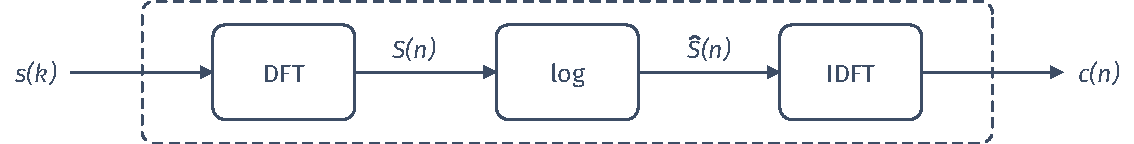
\includegraphics[width=0.9\textwidth]{./ch4-asr/img/cepstrum.pdf}
  \caption{Blokové schéma principu výpočtu kepstra}
  \label{fig:asr:model:speech:cepstrum}
\end{figure}

Pro získání kepstrálních koeficientů linearní predikce loagritmujeme rovnici (\ref{eq:asr:lpc:generic}) čímž vznikne vztah

\begin{equation}
  \log H(z) = \log \left( \frac{G}{A(z)} \right).
  \label{eq:asr:lpc:cepstrum}
\end{equation}

\noindent Člen $A(z)$ je polynomem proměnné $z^{-1}$ řádu $Q$, a pokud všechny jeho kořeny leží uvnitř jednotkové kružnice, tak lze aplikovat Taylorův rozvoj na vztah (\ref{eq:asr:lpc:cepstrum}) ve tvaru

\begin{equation}
  \log \left( \frac{G}{A(z)} \right) = c(0) + c(1)z^{-1} + \dots = \sum_{k=0}^{\infty} c(k)z^{-k},
  \label{eq:asr:lpc:cepstrum:taylor}
\end{equation}

\noindent kde $c(k)$ jsou tzv. kepstrální koeficienty LPC. K odstranění logaritmu je potřeba obě strany rovnice derivovat. Po úpravě je výsledný vztah

\begin{equation}
  - \sum_{i=1}^{Q} ia_iz^{-i} = \left( \sum_{k=0}^{\infty} kc(k)z^{-k} \right)\left( \sum_{i=0}^{Q} a_iz^{-i}\right).
  \label{eq:asr:lpc:cepstrum:deriv}
\end{equation}

\noindent Pokud se $a_i = 1$, pak je možné roznásobení rovnice (\ref{eq:asr:lpc:cepstrum:deriv}) a porovnání člený u stejných mocnin $z$ zapsat vztahy pro výpočet kepstrálních koeficientů LPC

\begin{align}
  \begin{split}
    c(1) &= -a_1, \\
    c(k) &=
    \begin{cases}
      - a_k - \sum_{i=1}^{k-1} \left(\frac{i}{k}\right) c(i) a_{k-1},  & \quad \text{pro } 2 \leq k \leq Q, \\
      - \sum_{i=1}^{Q} \left(\frac{k - i}{k}\right) c(k-i) a_i,  & \quad \text{pro } k = Q + 1, Q + 2, \dots \quad ,
    \end{cases}
  \end{split}
  \label{eq:asr:lpc:cepstrum:coef}
\end{align}

\noindent kde $k = 1, 2, \dots , Q^{*}$ a $Q^{*}$ je počet kepstrálních koeficientů a $Q^{*} \geq Q$.

Kepstrální koeficienty LPC jsou vztaženy ke spektrální obálce mikrosegmentu řeči odvozené LPC analýzou, tu je možné získat dosazením $e^{j\omega}$ za $z$ v rovnici (\ref{eq:asr:lpc:generic}). Pro uspokojivou reprezentaci se tradičně volí $Q = 7\ \text{až}\ 15$ v závislosti na spektrální šířce přenášeného pásma, požadované přesnosti aproximace apod. Z toho plyne, že pro popis mikrosegmentu řeči by mohl stačit příznakový vektor o $15$ koeficientech.

\subsection{Modelování procesu slyšení}
\label{chap:asr:parametrization:hearing}

Medelování procesu slyšení usilují o kompenzaci nelineárního vnímání frekvencí lidským sluchem. Dále pak i o respektování maskování zvuků včetně tzv. kritických pásem slyšení, což je přirozená vlastnost lidského sluchu. Maskováním se rozumí jev, kdy vnímání jednoho zvuku je ovlivněno přítomností jiného zvuku. Jinými slovy lze říci, že přitomnost jednoho zvuku zvyšuje práh slyšitelnosti pro jiný zvuk. Ten buď zní současně nebo s určitým časovým odstupem. Tento jev je jakýsi \uv{psychologický filtr}, který ignoruje věškerý šum ležící mimo určité kriticé pásmo. Šířka takového kritického pásma je přitom závislá na frekvenci poslouchaného tónu.

Typickým příkladem metod modelující proces slyšení jsou \textbf{melovská kepstrální filtrace} a \textbf{perceptivní lineární prediktivní analýza}.

\subsubsection{Melovské kepstrální koeficienty}

Metoda melovských frekvenčních kepstrálních koeficientů (MFCC) se snaží respoktovat výše zmíněné vlastnosti lidského sluchu. Zejména o dodržení kritických pásem slyšení a dále vlivu subjektivního vnímání výšky tónů.

Základem MFCC je využití banky filtrů a lineárním rozložením frekvencí v tzv. \textbf{melovské frekvenční škále} definované vztahem

\begin{equation}
  f_m = 2595 \log \left(1 + \frac{f}{700}\right),
  \label{eq:asr:mfcc:melscale}
\end{equation}

\noindent kde $f \left[Hz\right]$ je frekvence v lineární škále a $f_m \left[mel\right]$ je odpovídající frekvence v melovské škáleě. Melovský filtr má trojúhelníkový tvar. Banka obsahuje filtry rozmístěné lineárně v melovských frekvenčních souřanicích, a to tak, že dva sousední filtry se navzájem o polovinu překrývají. Pro střední frekvence jednotlivých filtrů $b_{m,i}$ platí v melovské škále vztah

\begin{equation}
  b_{m,i} = b_{m,i-1} + \Delta_{m},
  \label{eq:asr:mfcc:freq}
\end{equation}

\noindent kde $b_{m, 0} = 0\ mel$, $i = 1, 2,\ \dots\ , M^{*}$, a $\Delta_m = B_{m,w} / (M^{*} + 1)$. Ukázka banky filtrů je na obr. \ref{fig:asr:mfcc:bank:mel}. Pro výpočet odezvy filtrů je však nezbytné přepočítat všechny koeficienty FFT do melovské frekvenční škály. Vhodnější je vyjádření trjúhelníkových filtrů ve frekvenční škále s měřítkem v herzích.

\begin{figure}[hbpt]
  \centering
  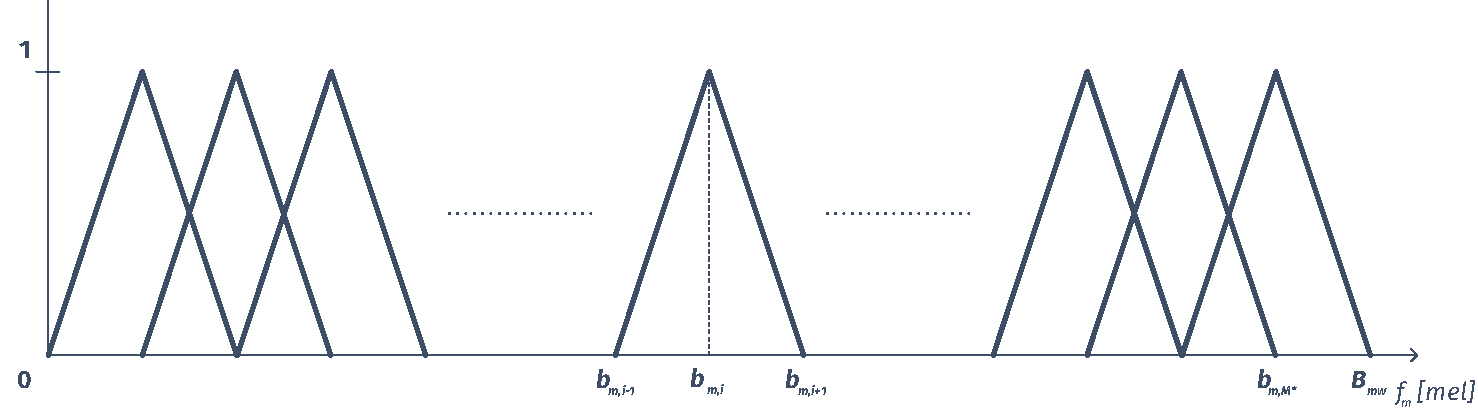
\includegraphics[width=0.9\textwidth]{./ch4-asr/img/filter_bank-mel.pdf}
  \caption{Rozložení banky trojúhelníkových filtrů v melovské frekvenční škále}
  \label{fig:asr:mfcc:bank:mel}
\end{figure}

\noindent K přepočtu středních frekvencí $b_{m,i}$ se využívá inverzního vztahu k (\ref{eq:asr:mfcc:melscale}) tedy

\begin{equation}
  f = 700 \left[ \exp\left( 0,887.10^{-3} f_m \right) - 1 \right].
  \label{eq:asr:mfcc:melscale:inverse}
\end{equation}

\noindent Střední frekvence $b_i,\ i=1,2,\ \dots\ , M^{*}+1$ jsou vyjádřené v jednozce $[Hz]$. Filtry jsou rozmístěny nelineárně viz obr. \ref{fig:asr:mfcc:bank:hz}.

\begin{figure}[hbpt]
  \centering
  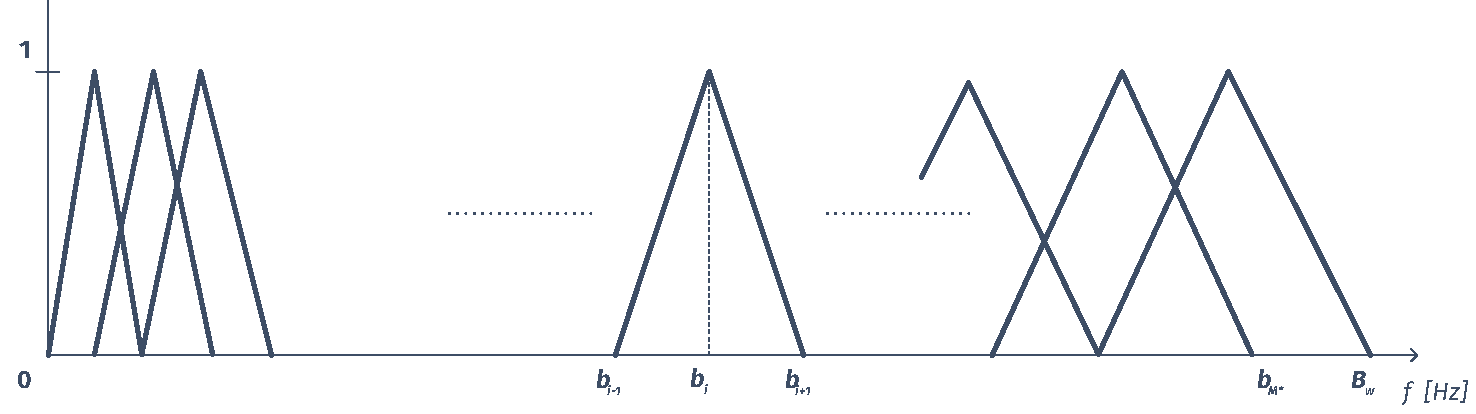
\includegraphics[width=0.9\textwidth]{./ch4-asr/img/filter_bank-hz.pdf}
  \caption{Rozložení banky trojúhelníkových filtrů ve frekvenční škále}
  \label{fig:asr:mfcc:bank:hz}
\end{figure}

Při výpočtu melovských kepstrálních koeficientů jsou na vstup systému přivedeny mikrosegmenty ($10$ až $30\ ms$) řečového signálu $s(k)$. Na vzorcích $s(k)$ byla ještě předtím provedena preemfáze\footnote{Preemfáze znamená zdůraznění amplitud spektrálních složek řečového signálu s jejich bzrůstající frekvencí. \cite{Psutka2006}}. Pro jednotlivé mikrosegmenty je pomocí FFT vypočteno amplitudové spektrum $\left| S(f) \right|$ a následuje klíčová část celého procesu, melovský filtrace. Odezvy filtrů ve frekvenční oblasti lze vyjádřit vztahem

\begin{equation}
  y_m(i) = \sum_{f=b_{i-1}}^{b_{i+1}} \left| S(f) \right| u\left(f, i\right),  \quad i = 1, 2,\ \dots\ ,M^{*},
  \label{eq:asr:mfcc:freq:responce}
\end{equation}

\noindent kde frekvence $f$ jsou vybírány ze souboru frekvencí využívaných při FFT výpočtu a $u(f, i)$ je vyjádření konkrétního troúhelníkového filtru $i$. Průchod filtrem tedy znamená, že každý koeficient FFt je násoben odpovídajícím ziskem filtru a výsledky jsou pro příslušné filtry akumulovány. Logaritomováním akumulovaných koeficientů $y_{m}(i)$ se provede převod do kepstrální oblasti. Tento krok příznivě omezí dynamiku signálu.

Posledním krokem při výpočtu melovských kepstrálních koeficientů $\left\{c_m\left(j\right)\right\}_{j=1}^{M}$ je provedení IDFT (viz (\ref{eq:asr:lpc:cepstrum:generic})). V případě MFCC se, ale používá diskrétní kosinova transformace (DCT), protože spektrum je reálné a symetrické. K výpočtu slouží vztah

\begin{equation}
  c_{m}(j) = \sum_{i=1}^{M^{*}} \log y_m(i) \cos\left( \frac{\pi j}{M^{*}}\left(i - 0,5\right) \right),  \quad \text{pro}\ j = 0, 1,\ \dots\ ,M,
  \label{eq:asr:mfcc:coef}
\end{equation}

\noindent kde $M^{*}$ je počet pásem melovkého pásmového filtru a $M$ je počet melovských kepstrálních koeficientů. Počet těchto koeficientů $M$ se volí podstatně menší, než je počet pásem melovského pásmového filtru $M^{*}$, obvykle se uvažuje prvních $M = 10\ \text{až}\ 13$ koeficientů.



